\documentclass{article}
\usepackage[utf8]{inputenc}
\usepackage{amsmath,amssymb}
\usepackage{graphicx}
\usepackage[a4paper,margin=0.9cm]{geometry}
\usepackage{multicol}
\usepackage{sectsty}

\graphicspath{ {.} }

\DeclareMathOperator{\ima}{Im}
\newcommand\tab[1][0,5cm]{\hspace*{#1}}

\begin{document}
	%\allsectionsfont{\small}
	%\scriptsize
	
	\mbox{}
	\vspace{10cm}
	\begin{center}
		\textbf{\Huge{Metal Oxide Field Effect Transistor}}\\
		\bigskip
		\Large{Tommaso Bertelli}\\
		\bigskip
		\Large{CO-526-B - Electronics Lab}\\
		\bigskip
		\Large{Instructor Uwe Pagel}\\
		\bigskip
		\Large{8/12/2024}\\
	\end{center}
	\pagebreak
	
	\section{Introduction - Prelab}
		\subsection{Metal Oxide Semiconductor Field Effect Transistors (MOSFET)}
			\begin{enumerate}
				\item 
				Enhancement MOSFET:
				- The transistor is normally off when no gate voltage is applied.
				- A positive (for NMOS) or negative (for PMOS) gate voltage is required to induce a conductive channel and turn it on.
				- Commonly used in modern electronics due to its low power consumption in the off state.\\
				Depletion MOSFET:		
				- The transistor is normally on without any gate voltage applied.
				- A gate voltage opposite to the type of the MOSFET (negative for NMOS, positive for PMOS) is applied to turn it off.
				- Less common compared to enhancement-mode MOSFETs.
				\item 
				NMOS Transistor:
				
				- Built using n-type material as the channel.
				- Requires a positive voltage at the gate relative to the source to turn it on.
				- Typically faster and has better electron mobility than PMOS.
				- Used for high-speed and high-performance applications.
				PMOS Transistor:
				
				- Built using p-type material as the channel.
				- Requires a negative voltage at the gate relative to the source to turn it on.
				- Slower than NMOS due to lower hole mobility.
				- Often used for low-power applications.
			\end{enumerate}
		\subsection{MOSFET as Amplifier}
			\begin{enumerate}
				\item 
				\(V_{GS} = V_G - V_S\), \(V_S = I_D \cdot R_S\)\\\\
				\(V_G = V_{DD} \cdot \frac{R_2}{R_1+R_2} \) = 5V\\\\
				Using the saturation current equation: \(I_D = k \cdot ((V_G - I_D \cdot R_S ) - V_{th})^2\)\\\\
				\(I_D \) = 0.888mA\\\\
				\(V_{DS} = V_{DD} - I_D(R_D + R_S) \) = -0.67V\\\\
				\(V_{GS} = V_G -V_S \) = -0.33V\\
				\item To verify that the MOSFET is in the saturation region \(V_DS\) must be greater than \(V_{GS} - V_{th}\)\\\\
				\(V_{DS}\) = -0.67V, \(V_{GS}\) = -0.33V, \(V_{th}\) = 1V, so the condition is verified.
			\end{enumerate}
		\subsection{MOSFET as Switch}
		\begin{enumerate}
			\item When \(U_{in}\) is 0V the mosfet is off, no current flows so \(V_{RD}\) = 0V and \(V_{DS} = V_{DD}\) = 10V.
			\item  From the graph, when \(V_{GS}\) is 2.4V, \(I_D \approx\) 55mA\\\\
			\(V_{DS} = V_{DD} - I_D \cdot R_D\) = 3.125V 
		\end{enumerate}\pagebreak
	\section{Experimental Set-up and Results}
		\subsection{ I/V Characteristic of a MOSFET}
			\begin{enumerate}
				\item Measured MOSFET transfer Characteristics\\\\
				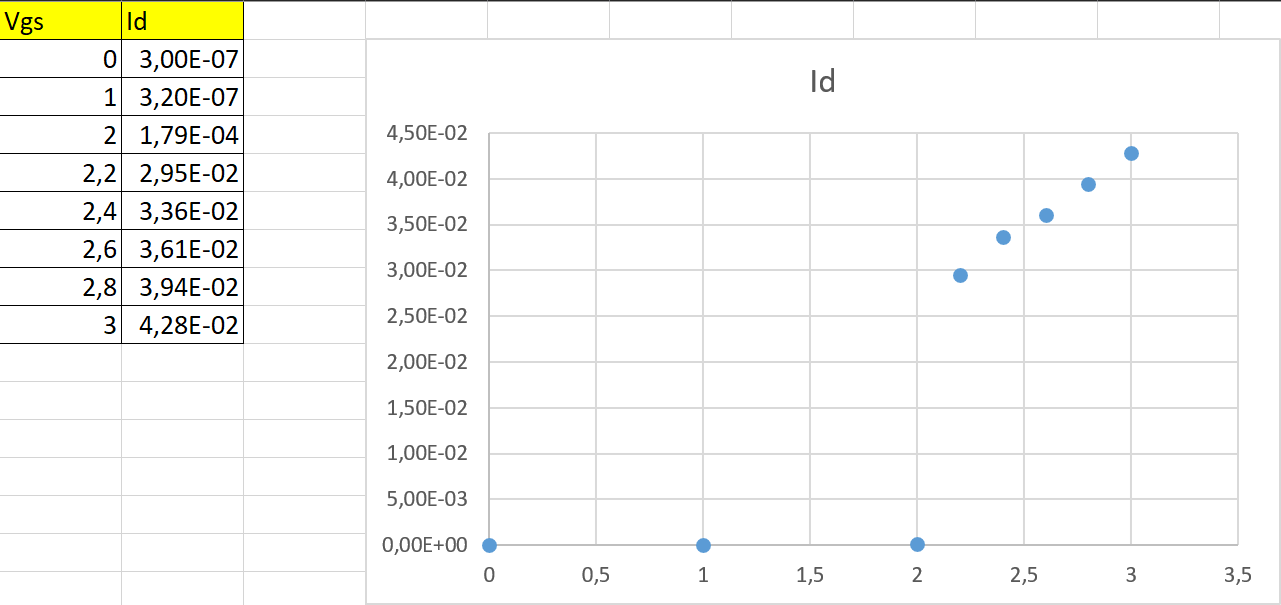
\includegraphics[scale=0.45]{graph 1}\\\\
				\item The measured \(V_{th}\) was 2.185V.\\
				The orange dot in the graphs represent the point (on the x-axis) where \(V_{DS} (V_{GS}-V_{th})\) is \(=\) 0.\\\\
				\(V_{GS} \) = 2V (under the threshold)\\\\
				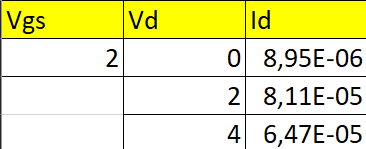
\includegraphics[scale=0.5]{graph 2}\\\\
				\(V_{GS} \) = 2.2V\\\\
				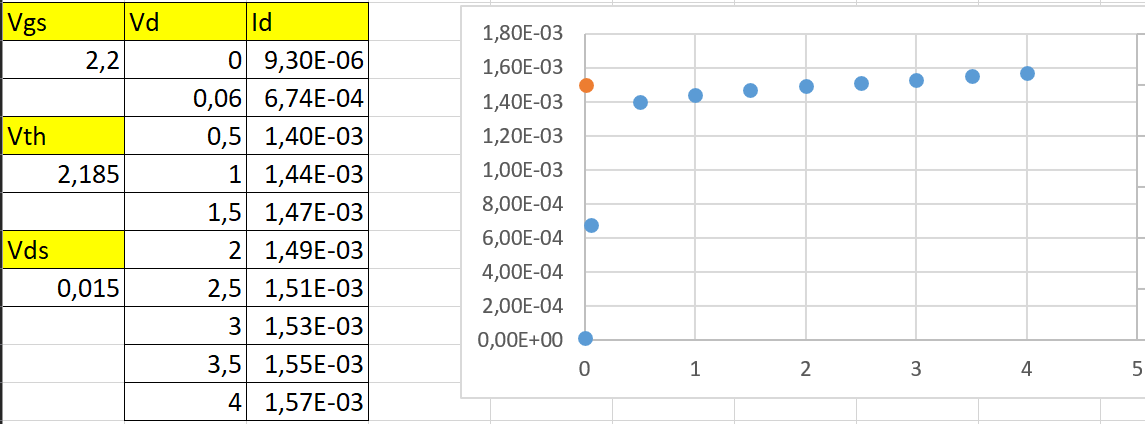
\includegraphics[scale=0.5]{graph 3}\pagebreak\\
				\(V_{GS} \) = 2.4V\\\\
				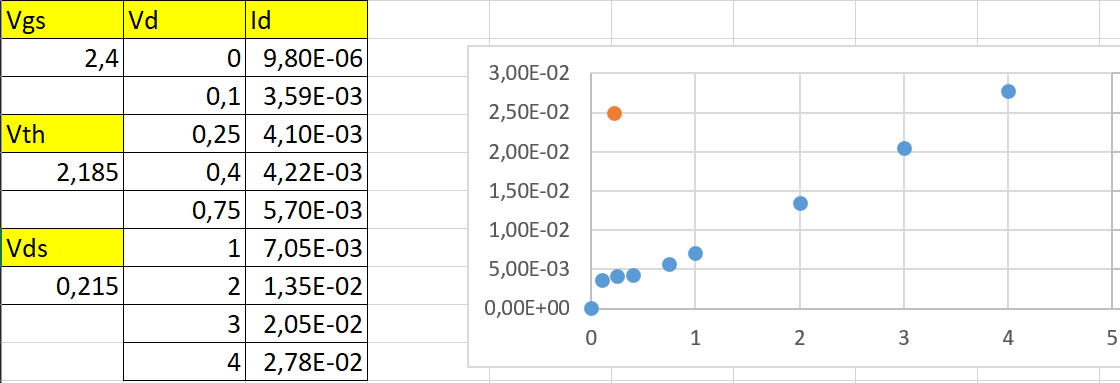
\includegraphics[scale=0.5]{graph 4}\\\\
				\(V_{GS} \) = 2.6V \\\\
				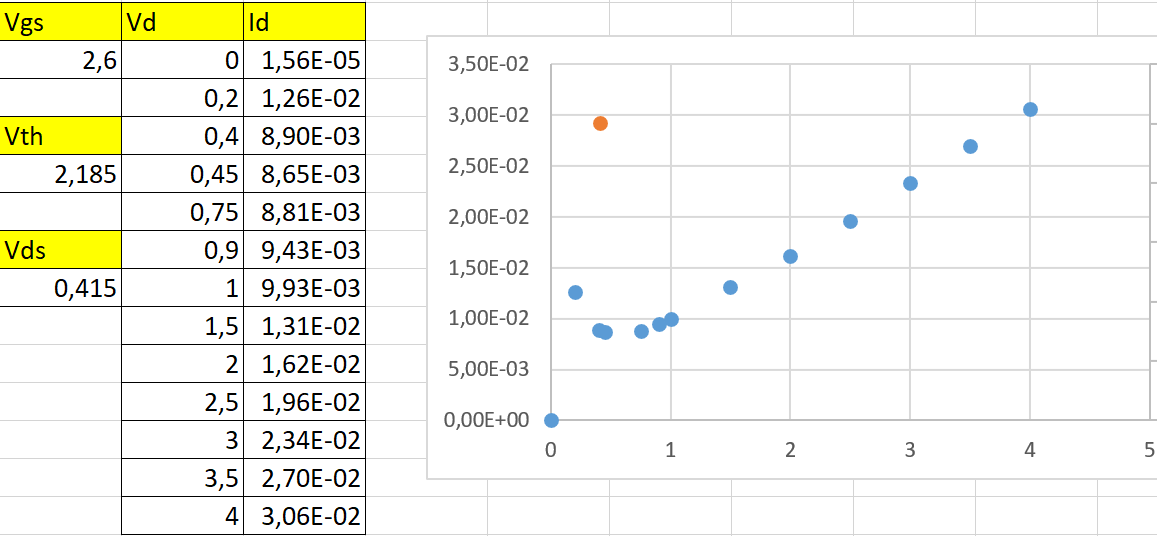
\includegraphics[scale=0.5]{graph 5}\\\\
				
				
			\end{enumerate}	
			
			
		\subsection{MOSFET as Amplifier}
			\begin{enumerate}
				\item  During amplification the MOSFET operates in saturation mode.\\
				This mode is ideal for amplification since the current \(I_D\) is primarly controlled by \(V_{GS}\) and the relationship between input and output is stable. The linear mode is not optimal for amplification since the MOSFET acts more as a resistor then as a controlled current source.
				
				\item Using the max \(V_{out} = V_{DD} =\) 10V and the min \(V_{out} =\)0V, the max clipping-free \(V_{in}\) = \(\frac{5V}{G}\) where \(G\) is the gain of the amplifier. 
				\item 
				Using the following formula to calculate the gain \(G = -2k R_D (V_{GS}-V_{th})\) and the provided and used values for \(R_D\) and \(k\), \(G\) =  17.1\\
				So the largest possigle input voltage amplitude usable without having clipping is 0.29V\\\\
				\pagebreak
				\item 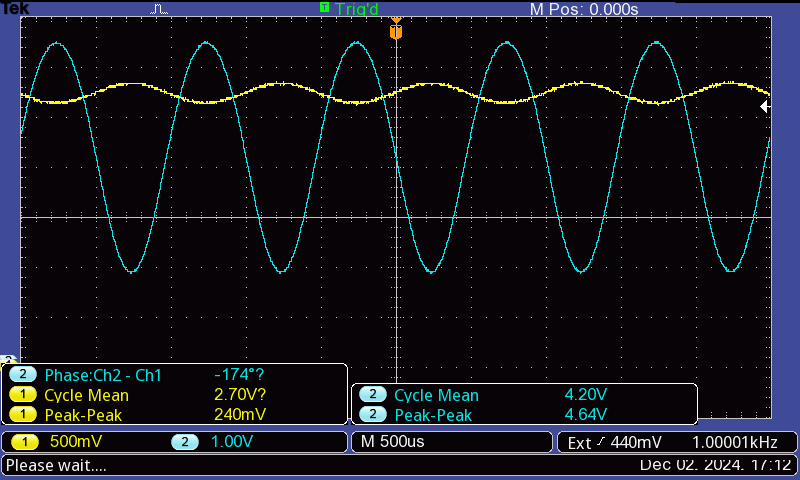
\includegraphics[scale=0.5]{F0011TEK}\\\\
				Input peak to peak voltage: 0.24V, output peak to peak voltage: 4.64V, Gain: 19.3, this value is a bit different from the theoretical one, this can be due to the different \(R_D\) used, to the physical transistor used and the different real \(k\) value.
				\item The output voltage is 180° phase shifted compared to the input voltage. This phase shift is due relationship between \(I_D\) and the output voltage \(V_{out}\). As \(I_D\) rises (along \(V_{in}\)), the voltage drop across \(R_D\) increases, pulling \(V_{out}\) closer to the ground. Because of this inverted relationship, there is a 180° phase shift between the input and output voltage.
				
			\end{enumerate}	\pagebreak
	
	
	\section{Lab 6 prelab}
		\subsection{Voltage Transfer Characteristic of a CMOS inverter}
			\begin{enumerate}
				\item 
				 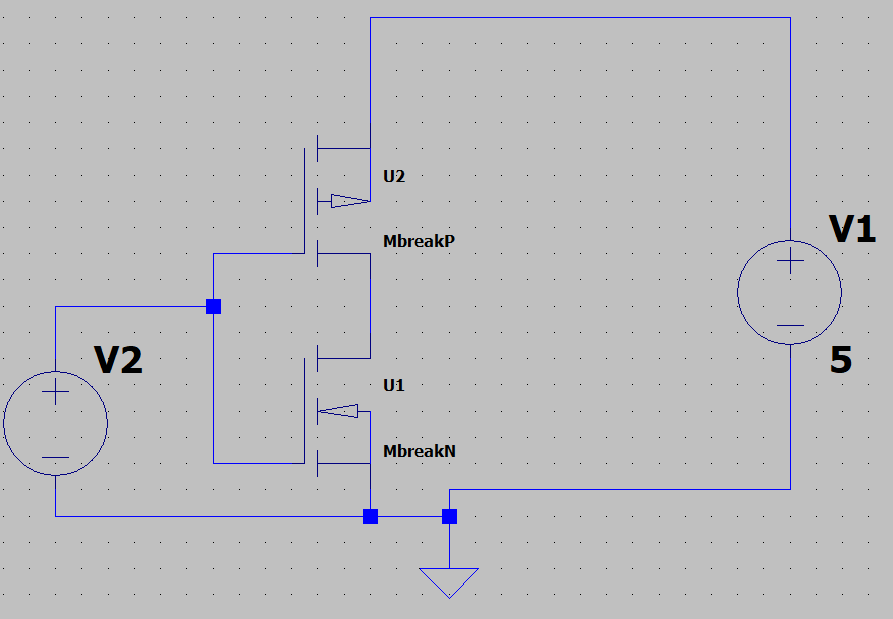
\includegraphics[scale=0.55]{prelab 6/2 circuit}\\\\
				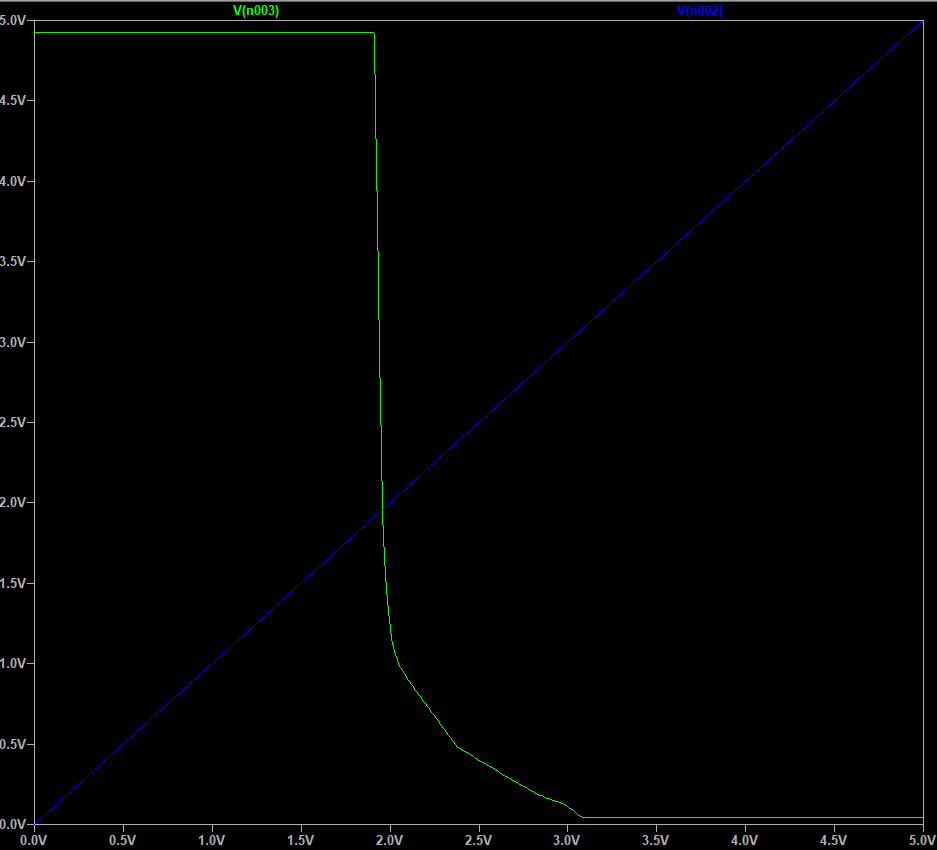
\includegraphics[scale=0.55]{prelab 6/1 vtc}\\\\
				Blue line: DC sweep of \(V_{in}\), Green line: \(V_{out}\)\\\\
				By measuring the graph: 
				\begin{itemize}
					\item \(V_{OH}\) = 4.93V
					\item \(V_{OL}\) = 40mV
					\item \(V_{th}\) = 1.96V
				\end{itemize}\pagebreak
				To measure \(V_{IH}\) and \(V_{IL}\) i plot \(d(V_{out})/d(V_{in})\)\\\\
				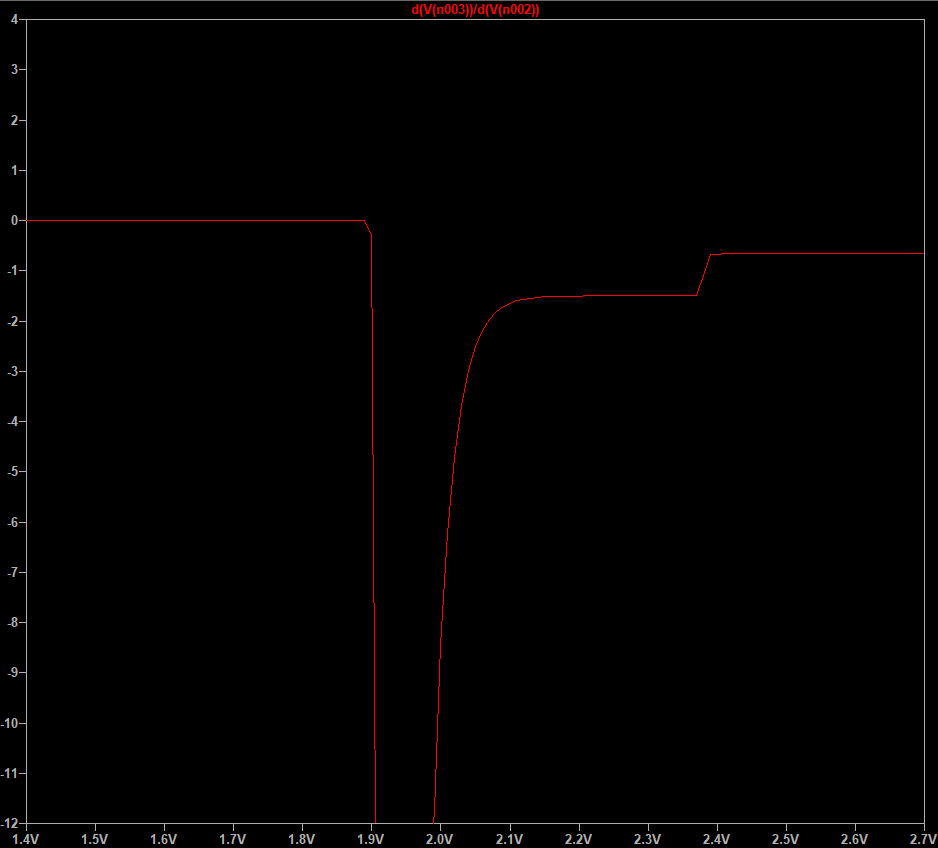
\includegraphics[scale=0.55]{prelab 6/1 deriv}\\\\
				\begin{itemize}
					\item \(V_{IH}\) = 2.38V
					\item \(V_{IL}\) = 1.91V
					\item \(NM_L\) = -3.02V
					\item \(NM_H\) = 2.34V
				\end{itemize}\pagebreak
			\item 
			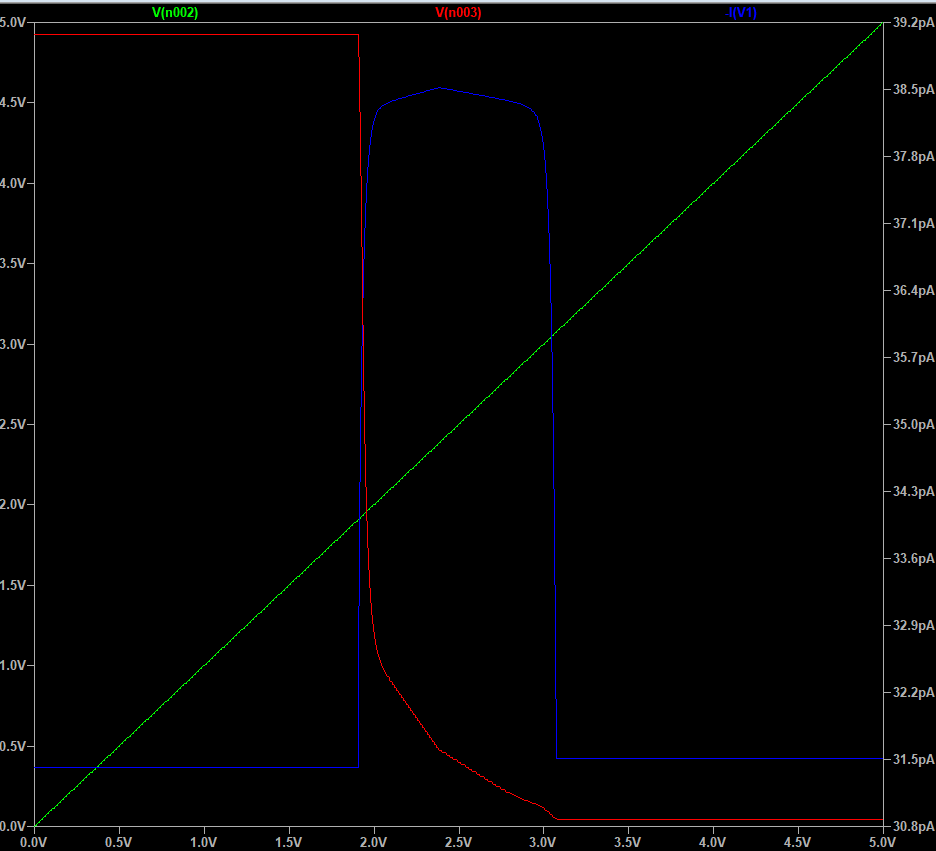
\includegraphics[scale=0.55]{prelab 6/1 curr}\\\\
			The blue line is the current through the inverter, the maximum is 38.5pA.
			\item The current reaches the maximum when the input level is 2.37V, this is due because both the NMOS and PMOS transistors are partially conducting, this happens around the transition region of the VTC curve. 
			\end{enumerate}
		\subsection{CMOS Inverter with Capacitive Load}	
			\begin{enumerate}
				\item Propagation delay for the different capacitors' values:
				\begin{itemize}
					\item 25pF: 96ns
					\item 50pF: 78ns
					\item 75pF: 67ns
					\item 100pF: 60ns
				\end{itemize}
				\item Power dissipation for the different capacitors' values:
				\begin{itemize}
					\item 25pF: 0.3125 \(\mu\)W
					\item 50pF: 0.625 \(\mu\)W
					\item 75pF: 0.9375 \(\mu\)W
					\item 100pF: 1.25 \(\mu\)W
				\end{itemize}
			\end{enumerate}
		\subsection{Propagation Delay of an Inverter Stage}
		\begin{enumerate}
			\item 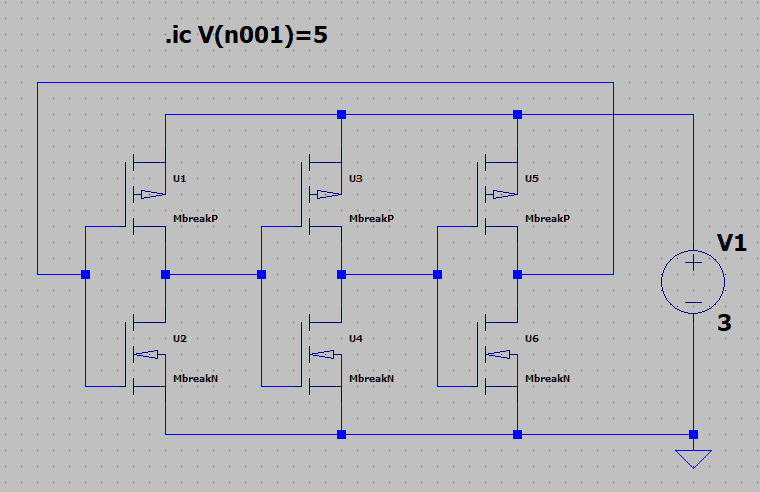
\includegraphics[scale=0.55]{prelab 6/3 circuit}\\\\
			The propagation delays and the oscillation frequencies of the ring oscillator at the different supply voltages are the following:
				\begin{itemize}
					\item 3V: 46.8ns, 7.5MHz
					\item 5V: 7.9ns, 42.8MHz
					\item 7V: 3.4ns, 98.1MHz
					\item 10V: 1.6ns, 211.7MHz
				\end{itemize}
			Example of measuring the oscillation frequency in the 10V case.\\\\
			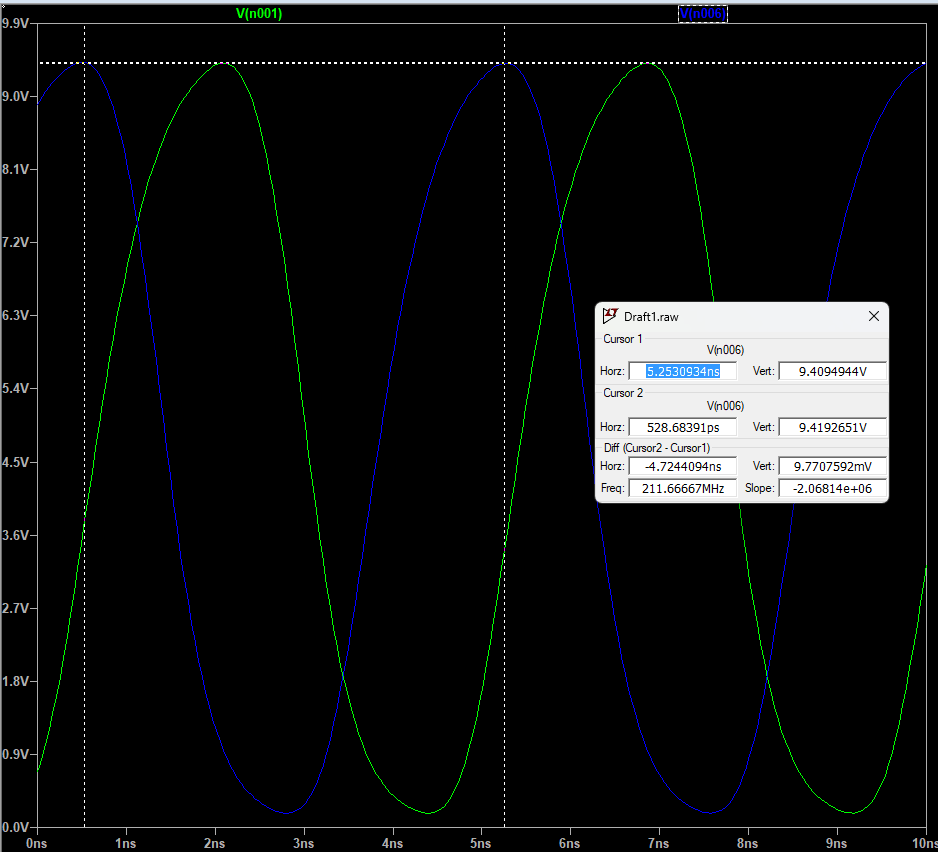
\includegraphics[scale=0.55]{prelab 6/3 freq}\\\\
			\item Behaviour of the ring oscillator with a 50pF capacitor added to each inverter stage.
			supply voltages.\\\\
			Propagation delay: 230ns, oscillation frequency: 1.44MHz, power dissipation: \(P_d=C_l\cdot V_{DD}^2 \cdot f\) = 1.8mW
			\item The presence of the capacitive load decreases the oscillation frequency and increases the propagation delay of the ring oscillator.
			\item According to the power dissipation formula, an increase on the capacitive load increases the power dissipation, and a linear increase on the supply voltage causes a quadratic increase in the power dissipation.
		\end{enumerate}
\end{document}
